%! Author = adrienkoumgangtegantchouang
%! Date = 09/06/25


\chapter{Deployment and Scaling}\label{ch:deployment-and-scaling}

This chapter covers containerized deployment for the Smart News Aggregator.


\section{Containerization with Docker}\label{sec:containerization-with-docker}


\subsection{Core Services Setup}\label{subsec:core-services-setup}

\begin{lstlisting}[style=bashstyle,label={lst:prometheus-configuration},caption={Prometheus Configuration (prometheus.yml)}]
global:
  scrape_interval: 15s

scrape_configs:
  - job_name: 'smart-news-aggregator-api'
    static_configs:
      - targets: ['smart-news-aggregator-api:5050']
      # - targets: ['localhost:5050']

  - job_name: 'redis'
    static_configs:
      - targets: ['redis-exporter:9121']

  - job_name: 'mongodb'
    static_configs:
      - targets: ['mongodb-exporter:9216']
\end{lstlisting}


\begin{lstlisting}[style=bashstyle,label={lst:docker-compose-core-services},caption={Docker compose for core services (docker-compose.yml)}]
services:
  redis:
    image: redis:alpine
    ports:
      - "6379:6379"
    volumes:
      - redis_data:/data
      - redis_backup:/backup
    command: redis-server --save 60 1 --loglevel warning
    restart: unless-stopped

  redis-exporter:
    image: oliver006/redis_exporter
    ports:
      - "9121:9121"
    environment:
      REDIS_ADDR: "redis://host.docker.internal:6379"

  mongodb:
    image: mongo:latest
    container_name: mongodb
    ports:
      - "27017:27017"
    volumes:
      - mongodb_data:/data/db
      - mongodb_backup:/backup
    platform: linux/arm64
    healthcheck:
      test: echo 'db.runCommand("ping").ok' | mongosh localhost:27017/test --quiet
      interval: 10s
      timeout: 10s
      retries: 5
    restart: unless-stopped

  mongodb-exporter:
    image: bitnami/mongodb-exporter:0.40.0
    ports:
      - "9216:9216"
    environment:
      MONGODB_URI: "mongodb://host.docker.internal:27017"

  prometheus:
    image: prom/prometheus
    ports:
      - "9090:9090"
    volumes:
      - ./prometheus.yml:/etc/prometheus/prometheus.yml

  grafana:
    image: grafana/grafana
    ports:
      - "3000:3000"
    volumes:
      - grafana_data:/var/lib/grafana
    depends_on:
      - prometheus

volumes:
  redis_data:
  redis_backup:
  mongodb_data:
  mongodb_backup:
  grafana_data:
\end{lstlisting}


\subsection{Backend Setup}\label{subsec:backend-setup}

\begin{lstlisting}[style=bashstyle,label={lst:dockerfile-backend},caption={Dockerfile Backend (Production configuration)}]
# Dockerfile.prod
FROM python:3.11-slim

WORKDIR /app

COPY requirements.txt .
RUN pip install --no-cache-dir -r requirements.txt

COPY . .

ENV FLASK_APP=src/app.py
ENV FLASK_ENV=production

EXPOSE 5000

# Use Gunicorn for production
CMD ["gunicorn", "-b", "0.0.0.0:5000", "src.app:application"]
\end{lstlisting}

\begin{lstlisting}[style=bashstyle,label={lst:docker-compose-backend},caption={Docker Compose Backend (docker-compose.yml)}]
services:
  smart-news-aggregator-api:
    build:
      context: .
      dockerfile: Dockerfile.prod
    ports:
      - "5050:5000"
    environment:
      - FLASK_ENV=production
      - FLASK_ENV_FILE=.env.prod
    env_file:
      - .env.prod
\end{lstlisting}


\subsection{Frontend Setup}\label{subsec:frontend-setup}

\begin{lstlisting}[style=bashstyle,label={lst:dockerfile-frontend},caption={Dockerfile Frontend (Production configuration)}]
# Stage 1: Build the Vite app
FROM node:20 as builder

WORKDIR /app

COPY package*.json ./
RUN npm install

COPY . .
RUN npm run build

# Stage 2: Serve with Nginx
FROM nginx:stable-alpine

# Copy the build output to Nginx web root
COPY --from=builder /app/dist /usr/share/nginx/html

# Optional: custom nginx config for single-page app (SPA)
COPY nginx.conf /etc/nginx/conf.d/default.conf

EXPOSE 80

CMD ["nginx", "-g", "daemon off;"]
\end{lstlisting}


\begin{lstlisting}[style=bashstyle,label={lst:docker-compose-frontend},caption={Docker Compose Frontend (docker-compose.yml)}]
services:
  smart-news-aggregator-fe:
    build:
      context: .
      dockerfile: Dockerfile.prod
    ports:
      - "3000:80" # host:container
\end{lstlisting}


\begin{lstlisting}[style=bashstyle,label={lst:},caption={ (.yml)}]

\end{lstlisting}


\section{Testing and Monitoring}\label{sec:testing-and-monitoring}

To ensure the reliability and correctness of the platform, the services were thoroughly tested and monitored after deployment.
All backend and frontend services were containerized using Docker, enabling isolated and consistent environments across development and production.

Once deployed, the services were interacted with directly through the exposed endpoints to verify the correct execution of key functionalities such as authentication,
article retrieval, comment posting, and admin operations (e.g., deleting users\cite{randomuser} or moderating content).
API responses were validated, edge cases were tested, and rate limits were checked.

Monitoring was achieved through an integrated dashboard, where metrics such as service uptime, API response times, error logs, and user activity were visualized.
This allowed real-time observation of system behavior and rapid identification of anomalies or performance bottlenecks.
Container logs were also inspected using docker logs and integration with monitoring tools like \textbf{Grafana} and \textbf{Prometheus}.



\section{Deployment Architecture Across Three Machines}\label{sec:deployment-architecture-across-three-machines}


The system has been deployed across three virtual machines within the same private network.
Each machine hosts a combination of services to ensure high availability, efficient resource distribution, and resilience.

For this deployment, I have this configuration:

\begin{tabularx}{\textwidth}{llX}
  \toprule
  Machine & IP Address & Services \\
  \midrule
  Machine 1 & 10.1.1.17 & MongoDB (Primary) + Redis Replica (Slave) \\
  Machine 2 & 10.1.1.18 & Redis Master + MongoDB (Slave) \\
  Machine 3 & 10.1.1.19 & Flask Backend API + React Frontend (Vite + Nginx) + Redis Sentinel (Monitoring) \\
  \bottomrule
\end{tabularx}

\begin{figure}[!h]
    \centering
    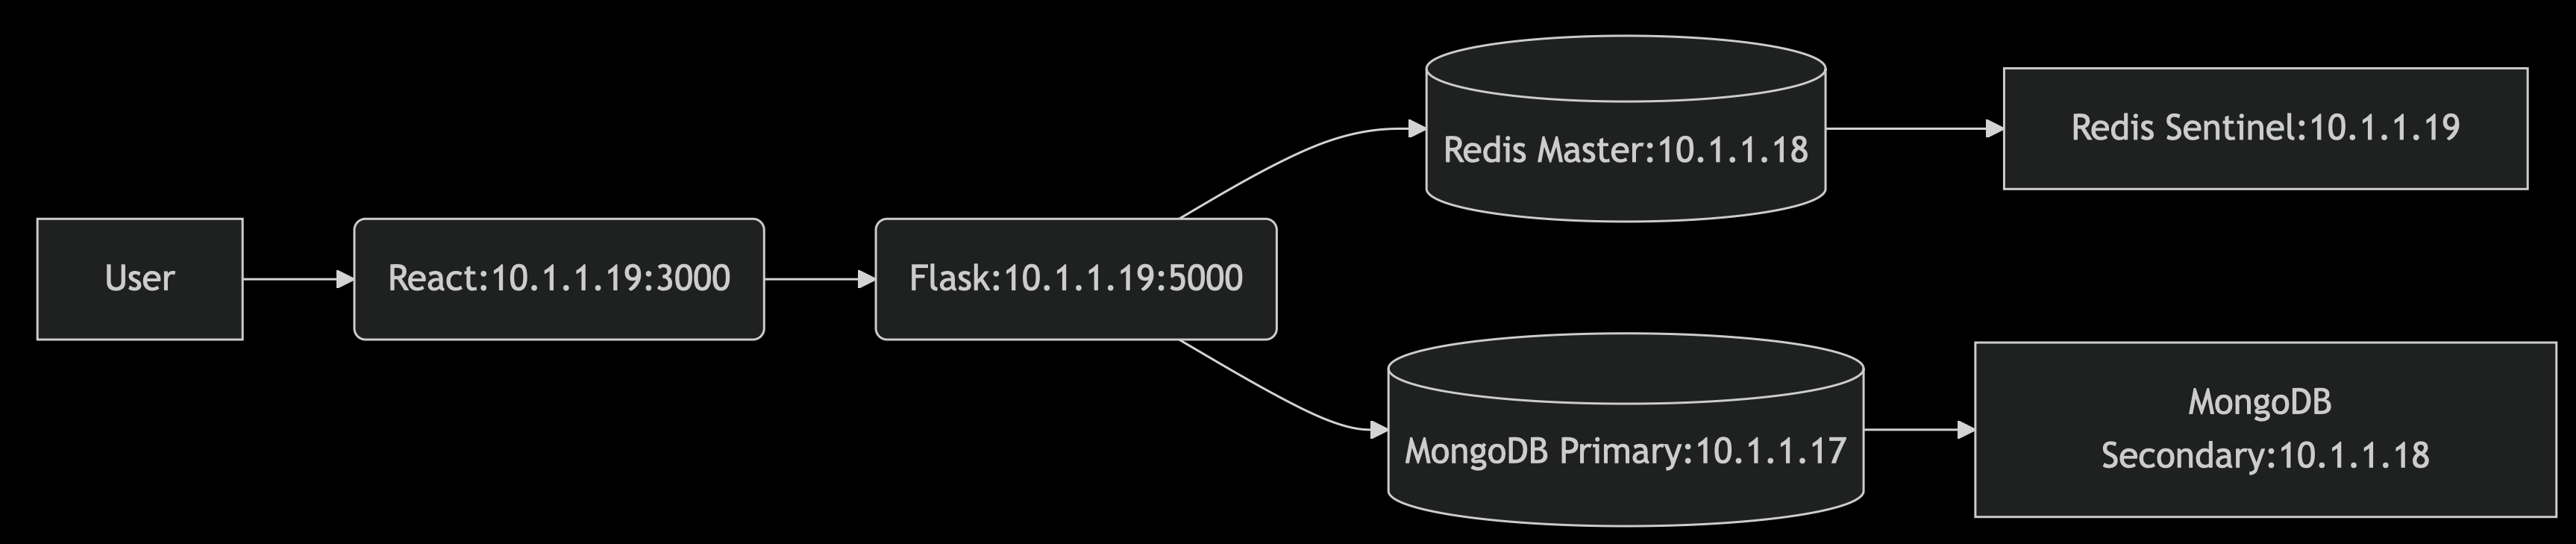
\includegraphics[width=1\textwidth]{chapters/chapter_08/deployment-vm-3}
    \caption{Deployment Architecture Accross Three Machines}
    \label{fig:deployment-vm-3}
\end{figure}

\subsection{MongoDB Replicat Set}\label{subsec:mongodb-replicat-set}

\textbf{MongoDB} is deployed as a replica set across Machines 1 and 2.

\begin{itemize}
  \item Primary (10.1.1.17) handles all write operations.
  \item Secondary (10.1.1.18) replicates the primary and allows read scalability.
  \item The backend connects using the replica set URI: $MONGODB\_URI=mongodb://10.1.1.17:27017,10.1.1.18:27017/?replicaSet=rs0$.
\end{itemize}

\subsection{Redis Replication + Sentinel}\label{subsec:redis-replication-+-sentinel}

Redis is set up with a master-slave configuration:

\begin{itemize}
  \item Master on 10.1.1.18.
  \item Replica (slave) on 10.1.1.17.
  \item Sentinel on 10.1.1.19 monitors the Redis master and handles automatic failover.
  \item Now, the backend is directly connected to the master.
\end{itemize}

\subsection{Flask Backend}\label{subsec:flask-backend}

The Flask API backend is hosted on Machine 3 (10.1.1.19).
It connects to MongoDB and Redis using internal IPs.

It's launched in production using \textbf{Gunicorn}, with the following environment configuration:


\begin{lstlisting}[style=bashstyle,label={lst:flask-api-backend-environment},caption={Flask API Backend Environment}]
FLASK_APP=src/app.py
FLASK_ENV=production
MONGODB_URI=mongodb://10.1.1.17:27017,10.1.1.18:27017/?replicaSet=rs0
REDIS_URL=redis://10.1.1.18:6379
\end{lstlisting}

Deployment steps from ./run-flask-prod.sh:

\begin{lstlisting}[style=bashstyle,label={lst:flask-backend-deployment-step},caption={Flask Backend Deployment Step}]
#!/bin/bash

# Exit if any command fails
set -e

# Define your project root (adjust this if needed)
PROJECT_DIR=$(dirname "$0")

cd "$PROJECT_DIR"

# Set environment variables
export FLASK_APP=src/app.py
export FLASK_ENV=production
export FLASK_ENV_FILE=.env.prod

# Clean existing virtual environment
rm -rf .venv

python3.13 -m venv --without-pip .venv

# Activate virtual environment
source .venv/bin/activate
curl -sS https://bootstrap.pypa.io/get-pip.py | python

# Install dependencies
pip install --upgrade pip
pip install --no-cache-dir -r requirements.txt

# Run using Gunicorn (you can change workers if needed)
gunicorn -b 0.0.0.0:5000 src.app:application

\end{lstlisting}

\subsection{React Frontend}\label{subsec:react-frontend}

The React app is built using \textbf{Vite} and served via \textbf{Nginx} on port 3000 on Machine 3.

It reads the base API URL at build time via .env:
\begin{lstlisting}[style=bashstyle,label={lst:react-frontend-environment},caption={React Frontend Environment}]
VITE_BASE_URL_API=http://10.1.1.19:5000
\end{lstlisting}

Deployment steps:

\begin{lstlisting}[style=bashstyle,label={lst:react-frontend-deployment-step},caption={React Frontend Deployment Step}]
  npm install
  npm run build
  npm start
\end{lstlisting}


The frontend app is available locally via ssh on
\begin{lstlisting}[style=bashstyle,label={lst:react-frontend-access-ssh},caption={React Frontend Access via SSH Command}]
ssh -N -L 3000:localhost:3000 root@10.1.1.19
\end{lstlisting}



